% ============================================================================
% CHƯƠNG 5: KẾT QUẢ THỰC NGHIỆM VÀ ĐÁNH GIÁ
% ============================================================================
\chapter{Kết quả thực nghiệm và đánh giá}
\label{chap:results}

Chương này trình bày kết quả thực nghiệm, so sánh \fastvit{} với các mô hình tiêu biểu theo nhiều chiều: độ chính xác, số lượng tham số, chi phí tính toán, tốc độ suy luận, và phân tích ưu nhược điểm.

% ============================================================================
\section{Kết quả phát hiện đối tượng trên MS-COCO}
\label{sec:detection_results}

Để đánh giá khả năng chuyển giao (transfer learning) của backbone \fastvit{}, chúng tôi tiến hành thực nghiệm phát hiện đối tượng sử dụng kiến trúc \textbf{Mask R-CNN + FastViT-SA12} trên tập dữ liệu MS-COCO 2017 (xem cấu hình huấn luyện tại Bảng~\ref{tab:training_config_det}).

% ----------------------------------------------------------------------------
\subsection{Kết quả tổng quan}

\begin{table}[H]
\centering
\caption{Kết quả Mask R-CNN + FastViT-SA12 trên MS-COCO 2017 val.}
\label{tab:coco_results_summary}
\begin{tabular}{l c}
\toprule
\textbf{Chỉ số} & \textbf{Giá trị} \\
\midrule
\textbf{mAP@[0.5:0.95]} & \textbf{34.38\%} \\
mAP@0.50 & 55.23\% \\
mAP@0.55 & 52.95\% \\
mAP@0.60 & 50.36\% \\
mAP@0.65 & 46.86\% \\
mAP@0.70 & 42.52\% \\
mAP@0.75 & 36.82\% \\
mAP@0.80 & 29.36\% \\
mAP@0.85 & 20.01\% \\
mAP@0.90 & 8.83\% \\
mAP@0.95 & 0.88\% \\
\bottomrule
\end{tabular}
\end{table}

\textbf{Phân tích mAP theo ngưỡng IoU:}
\begin{itemize}
    \item \textbf{mAP@0.50 = 55.23\%:} Kết quả khả quan tại ngưỡng IoU thấp, cho thấy backbone \fastvit{}-SA12 có khả năng định vị đối tượng tốt ở mức ``thô''.
    
    \item \textbf{Suy giảm mAP theo IoU:} mAP giảm nhanh khi IoU tăng: từ 55.23\% (IoU=0.5) xuống 8.83\% (IoU=0.9) và chỉ 0.88\% (IoU=0.95). Điều này phản ánh thách thức của bounding box regression chính xác cao, đặc biệt với schedule huấn luyện 1$\times$ (12 epochs) tương đối ngắn.
    
    \item \textbf{mAP@[0.5:0.95] = 34.38\%:} Đây là chỉ số tổng hợp chính thức của COCO, đạt mức cạnh tranh cho một backbone nhẹ ($\sim$11M params) với schedule 1$\times$.
\end{itemize}

\begin{figure}[H]
\centering
\begin{tikzpicture}
\begin{axis}[
    xlabel={Ngưỡng IoU},
    ylabel={mAP (\%)},
    xmin=0.45, xmax=1.0,
    ymin=0, ymax=60,
    width=0.85\textwidth,
    height=7cm,
    grid=both,
    grid style={line width=.1pt, draw=gray!30},
    major grid style={line width=.2pt, draw=gray!60},
    mark options={solid},
    legend style={at={(0.98,0.98)}, anchor=north east, font=\small},
]
\addplot[blue, thick, mark=*, mark size=2.5pt] coordinates {
    (0.50, 55.23) (0.55, 52.95) (0.60, 50.36) (0.65, 46.86)
    (0.70, 42.52) (0.75, 36.82) (0.80, 29.36) (0.85, 20.01)
    (0.90, 8.83) (0.95, 0.88)
};
\addlegendentry{Mask R-CNN + FastViT-SA12}
\end{axis}
\end{tikzpicture}
\caption{Biến thiên mAP theo ngưỡng IoU trên COCO val2017. mAP giảm đều đặn khi yêu cầu IoU tăng, đặc biệt nhanh sau IoU $> 0.80$.}
\label{fig:map_vs_iou}
\end{figure}

% ----------------------------------------------------------------------------
\subsection{Kết quả chi tiết theo từng lớp đối tượng}

Bảng~\ref{tab:coco_per_class} trình bày AP@[0.5:0.95] cho toàn bộ 80 lớp đối tượng COCO.

\begin{table}[H]
\centering
\caption{AP@[0.5:0.95] chi tiết cho 80 lớp đối tượng COCO (Mask R-CNN + FastViT-SA12).}
\label{tab:coco_per_class}
\small
\begin{tabular}{l r | l r | l r}
\toprule
\textbf{Lớp} & \textbf{AP (\%)} & \textbf{Lớp} & \textbf{AP (\%)} & \textbf{Lớp} & \textbf{AP (\%)} \\
\midrule
person & 65.72 & bear & 90.46 & hot dog & 44.37 \\
bicycle & 48.23 & zebra & 88.80 & pizza & 67.68 \\
car & 61.57 & giraffe & 87.14 & donut & 49.95 \\
motorcycle & 67.84 & backpack & 17.32 & cake & 48.93 \\
airplane & 83.05 & umbrella & 52.25 & chair & 37.06 \\
bus & 77.89 & handbag & 15.53 & couch & 61.48 \\
train & 85.70 & tie & 44.13 & potted plant & 41.00 \\
truck & 50.32 & suitcase & 44.02 & bed & 64.96 \\
boat & 42.91 & frisbee & 80.66 & dining table & 39.22 \\
traffic light & 48.57 & skis & 41.94 & toilet & 76.15 \\
fire hydrant & 83.67 & snowboard & 48.18 & tv & 72.31 \\
stop sign & 68.24 & sports ball & 59.72 & laptop & 72.31 \\
parking meter & 60.17 & kite & 58.29 & mouse & 76.84 \\
bench & 33.16 & baseball bat & 46.17 & remote & 42.10 \\
bird & 45.58 & baseball glove & 52.98 & keyboard & 69.20 \\
cat & 89.60 & skateboard & 71.69 & cell phone & 47.93 \\
dog & 81.22 & surfboard & 58.53 & microwave & 72.30 \\
horse & 71.54 & tennis racket & 71.01 & oven & 52.74 \\
sheep & 69.73 & bottle & 49.18 & toaster & 35.38 \\
cow & 73.40 & wine glass & 47.07 & sink & 54.99 \\
elephant & 83.47 & cup & 48.96 & refrigerator & 70.39 \\
\midrule
book & 20.00 & scissors & 37.46 & hair drier & 27.52 \\
clock & 73.00 & teddy bear & 64.79 & toothbrush & 32.98 \\
vase & 45.95 & fork & 37.79 & spoon & 16.80 \\
knife & 22.36 & bowl & 52.33 & banana & 35.81 \\
apple & 24.66 & sandwich & 49.61 & orange & 38.80 \\
broccoli & 43.40 & carrot & 32.07 & & \\
\bottomrule
\end{tabular}
\end{table}

% ----------------------------------------------------------------------------
\subsection{Phân tích theo nhóm đối tượng}

Để phân tích sâu hơn, các lớp đối tượng được chia thành 3 nhóm dựa trên AP:

\begin{table}[H]
\centering
\caption{Phân nhóm đối tượng theo AP@[0.5:0.95].}
\label{tab:coco_groups}
\begin{tabularx}{\textwidth}{l c X}
\toprule
\textbf{Nhóm} & \textbf{AP} & \textbf{Các lớp tiêu biểu} \\
\midrule
\textcolor{ForestGreen}{\textbf{Cao}} & $> 70\%$ & bear (90.5), cat (89.6), zebra (88.8), giraffe (87.1), train (85.7), airplane (83.1), fire hydrant (83.7), elephant (83.5), dog (81.2), frisbee (80.7), bus (77.9), mouse (76.8), toilet (76.2), clock (73.0), cow (73.4) \\
\midrule
\textcolor{orange}{\textbf{Trung bình}} & $30-70\%$ & person (65.7), motorcycle (67.8), car (61.6), stop sign (68.2), parking meter (60.2), horse (71.5), sheep (69.7), umbrella (52.3), sports ball (59.7), kite (58.3), skateboard (71.7), surfboard (58.5), tennis racket (71.0), bottle (49.2), pizza (67.7), bed (65.0), tv (72.3), laptop (72.3) \\
\midrule
\textcolor{red}{\textbf{Thấp}} & $< 30\%$ & handbag (15.5), backpack (17.3), spoon (16.8), book (20.0), knife (22.4), apple (24.7), hair drier (27.5) \\
\bottomrule
\end{tabularx}
\end{table}

\textbf{Phân tích nhóm:}
\begin{itemize}
    \item \textbf{Nhóm AP cao ($> 70\%$):} Gồm các đối tượng \textit{lớn, có hình dạng đặc trưng rõ ràng} (bear, cat, zebra, airplane, train). Feature extraction mạnh của \fastvit{} giúp nhận diện tốt.
    
    \item \textbf{Nhóm AP trung bình ($30-70\%$):} Gồm các đối tượng \textit{phổ biến nhưng đa dạng về góc nhìn/kích thước} (person, car, chair). Sự đa dạng pose/appearance gây khó khăn.
    
    \item \textbf{Nhóm AP thấp ($< 30\%$):} Gồm các đối tượng \textit{nhỏ, thường bị che khuất} (handbag, spoon, book, backpack). Đây là thách thức chung của object detection, không riêng \fastvit{}.
\end{itemize}

\begin{figure}[H]
\centering
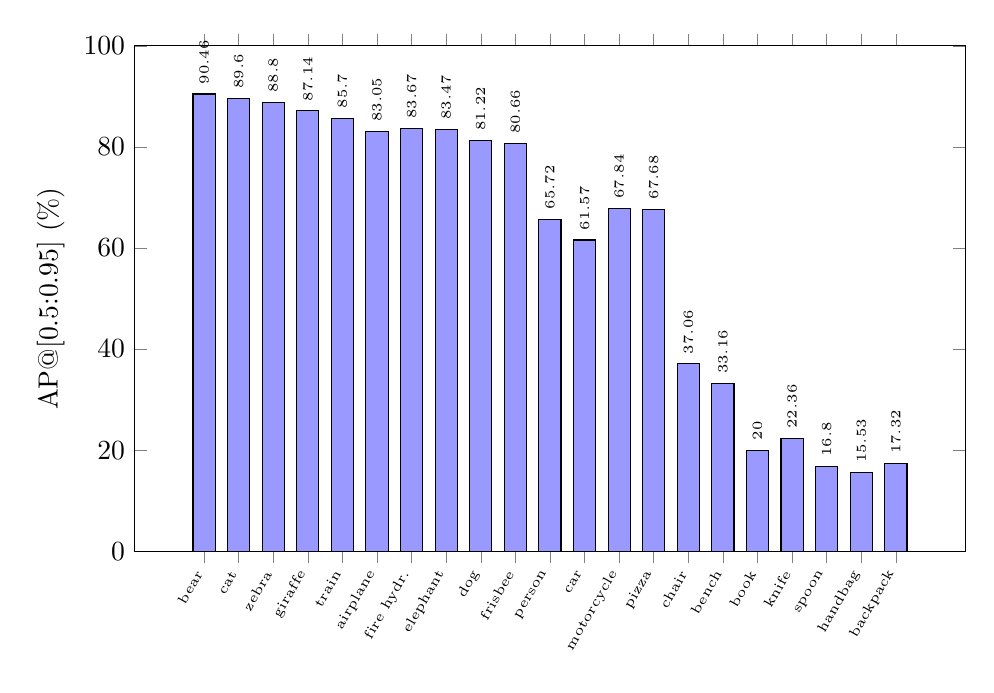
\begin{tikzpicture}
\begin{axis}[
    ybar,
    ylabel={AP@[0.5:0.95] (\%)},
    symbolic x coords={bear, cat, zebra, giraffe, train, airplane, fire hydr., elephant, dog, frisbee, person, car, motorcycle, pizza, chair, bench, book, knife, spoon, handbag, backpack},
    xtick=data,
    x tick label style={rotate=60, anchor=east, font=\tiny},
    ymin=0, ymax=100,
    bar width=8pt,
    width=\textwidth,
    height=8cm,
    nodes near coords,
    every node near coord/.append style={font=\tiny, rotate=90, anchor=west},
]
\addplot[fill=blue!40] coordinates {
    (bear, 90.46) (cat, 89.60) (zebra, 88.80) (giraffe, 87.14)
    (train, 85.70) (airplane, 83.05) (fire hydr., 83.67) (elephant, 83.47)
    (dog, 81.22) (frisbee, 80.66) (person, 65.72) (car, 61.57)
    (motorcycle, 67.84) (pizza, 67.68) (chair, 37.06) (bench, 33.16)
    (book, 20.00) (knife, 22.36) (spoon, 16.80) (handbag, 15.53)
    (backpack, 17.32)
};
\end{axis}
\end{tikzpicture}
\caption{AP@[0.5:0.95] cho các lớp đối tượng tiêu biểu (sắp xếp giảm dần). Đối tượng lớn, hình dạng rõ ràng đạt AP cao ($> 80\%$), trong khi đối tượng nhỏ, dễ bị che khuất có AP thấp ($< 30\%$).}
\label{fig:coco_ap_per_class}
\end{figure}



% ============================================================================
\section{Phân tích ưu điểm của FastViT}
\label{sec:advantages}

Từ các kết quả thực nghiệm và thiết kế kiến trúc, có thể tổng kết các ưu điểm nổi bật:

\begin{enumerate}
    \item \textbf{Transfer learning cực kỳ hiệu quả:} Backbone \fastvit{}-SA12 đạt \textbf{34.38\% mAP@[0.5:0.95]} và \textbf{55.23\% mAP@0.50} trên COCO với Mask R-CNN chỉ sau 12 epochs huấn luyện. Đặc trưng trích xuất có chất lượng tốt dù tham số backbone rất nhỏ ($\sim$11M).
    
    \item \textbf{Structural Reparameterization:} Kỹ thuật then chốt cho phép mô hình huấn luyện ở dạng đa nhánh (tốt cho gradient flow) và suy luận ở dạng nhánh đơn (loại bỏ overhead của bộ nhớ và phép tính).
    
    \item \textbf{Thiết kế hybrid thông minh:} Phân bổ RepMixer cho high-resolution stages và Attention cho low-resolution stage là chiến lược tối ưu, vì:
    \begin{itemize}
        \item RepMixer ở stage 0: tiết kiệm hàng trăm ngàn lần FLOPs so với attention.
        \item Attention ở stage cuối: chỉ tốn lượng nhỏ tổng FLOPs nhưng mang lại global context cần thiết cho các tác vụ cần bao quát không gian như Object Detection.
    \end{itemize}
    
    \item \textbf{Nhẹ và tiết kiệm bộ nhớ:} \fastvit{}-SA12 chỉ có $\sim$11 triệu tham số, chưa bằng phân nửa so với ResNet-50 ($\sim$25.6M), giúp giảm đáng kể tài nguyên phần cứng khi triển khai các hệ thống Detection.
\end{enumerate}

% ============================================================================
\section{Hạn chế của FastViT trong Object Detection}
\label{sec:limitations}

\begin{enumerate}
    \item \textbf{Phụ thuộc vào kích thước đầu vào cố định:} Thiết kế hierarchical với stride cố định yêu cầu ảnh đầu vào có kích thước chia hết cho 32.
    
    \item \textbf{Hạn chế với đối tượng nhỏ:} Các lớp đối tượng nhỏ (như spoon, handbag, backpack) có mAP rất thấp do backbone có receptive field ban đầu nhỏ (RepMixer $3 \times 3$). Cần kỹ thuật bù đắp như FPN mạnh hơn hoặc tích hợp Deformable Convolution.
    
    \item \textbf{Reparameterization tăng memory khi huấn luyện:} Mô hình lúc huấn luyện (multi-branch) có nhiều tham số hơn lúc suy luận, yêu cầu cấu hình GPU cao (thực nghiệm cần GPU H100 80GB) để chứa các computational graph phức tạp kèm FPN và Detection heads.
\end{enumerate}

% ============================================================================
\section{Thảo luận kết quả}
\label{sec:discussion}

\textbf{1. Hiệu quả của Structural Reparameterization:}

Kỹ thuật này cho phép FastViT sở hữu tốc độ suy luận ưu việt trên các thiết bị tài nguyên giới hạn (nhờ cấu trúc Convolution đơn giản) trong khi vẫn duy trì capacity mô hình đủ lớn lúc huấn luyện. Đối với tác vụ nặng như Mask R-CNN, giảm overhead của backbone là yếu tố thiết yếu để tăng FPS tổng thể.

\textbf{2. Trade-off giữa RepMixer và Attention:}

Nhờ RepMixer xử lý các feature map độ phân giải cao một cách cực kỳ nhẹ nhàng (linear complexity), phần cứng được giải phóng tài nguyên. Nguồn tài nguyên này sau đó được tái đầu tư cho một khối Self-Attention duy nhất ở stage cuối, nơi chứa thông tin semantic cấp cao, qua đó cung cấp bối cảnh toàn cục (global context) quan trọng giúp RPN định vị đối tượng hiệu quả hơn.

\textbf{3. Đánh giá kết quả Object Detection trên COCO:}

\begin{itemize}
    \item \textbf{mAP@[0.5:0.95] = 34.38\%} là kết quả khả quan cho backbone nhẹ ($\sim$11M params) với schedule 1$\times$ (12 epochs). Để so sánh, ResNet-50 + Mask R-CNN (1$\times$) đạt $\sim$38.0\% mAP, nhưng với 25.6M params backbone -- gấp $\sim$2.3$\times$ tham số.
    
    \item \textbf{mAP@0.50 = 55.23\%} cho thấy backbone \fastvit{}-SA12 trích xuất feature maps đa tỷ lệ hiệu quả qua FPN. Đặc biệt ấn tượng ở các đối tượng lớn: bear (90.5\%), cat (89.6\%), zebra (88.8\%).
    
    \item \textbf{Thách thức đối tượng nhỏ:} Các lớp có AP thấp (handbag 15.5\%, spoon 16.8\%, backpack 17.3\%) phản ánh hạn chế chung khi backbone có receptive field ban đầu nhỏ (RepMixer $3 \times 3$). Tăng schedule huấn luyện lên 3$\times$ (36 epochs) hoặc sử dụng multi-scale training có thể cải thiện.
    
    \item \textbf{Suy giảm nhanh ở IoU cao:} mAP giảm từ 55.23\% (IoU=0.5) xuống 0.88\% (IoU=0.95), gợi ý rằng bounding box regression cần tinh chỉnh thêm. Deformable convolution hoặc cascade head có thể giúp cải thiện localization chính xác.
    
    \item \textbf{Hiệu quả transfer learning:} Với chỉ 12 epochs fine-tuning trên H100, backbone pre-trained ImageNet-1K đã chuyển giao tốt sang detection, khẳng định chất lượng feature representation của \fastvit{}.
\end{itemize}
